\documentclass[tikz]{standalone}
\usepackage{pgfplots}
\pgfplotsset{compat=1.15}
\usepackage{mathrsfs}
\usetikzlibrary{arrows,calc}
\usepackage{tkz-euclide}
\pagestyle{empty}

\definecolor{AngleClr}{rgb}{0,0.39215686274509803,0}
\definecolor{ShapeClr}{rgb}{0.6,0.2,0}
\definecolor{SquareClr}{RGB}{250, 248, 217}


\begin{document}

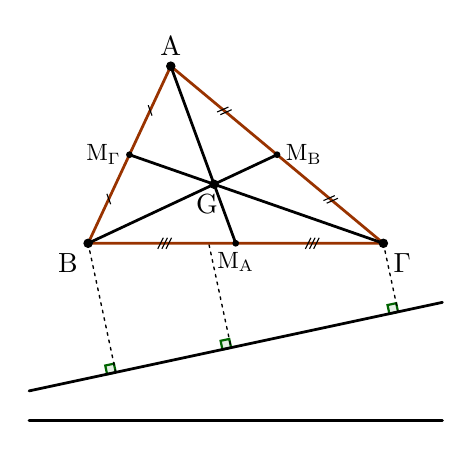
\begin{tikzpicture}[scale=.75]
\tkzSetUpLine[line width=1pt,color=black]
\tkzSetUpPoint[fill=black]

\tkzDefPoints{0/0/B,1.4/3/A,5/0/C}
\tkzDefPoints{-1/-2.5/E,6/-1/EE}

\tkzDefPoints{-1/-3/X,6/-3/XX}

\tkzDefMidPoint(B,C) \tkzGetPoint{MA}
\tkzDefMidPoint(A,C) \tkzGetPoint{MB}
\tkzDefMidPoint(A,B) \tkzGetPoint{MC}

\tkzDefPointBy[projection=onto E--EE](A)\tkzGetPoint{PA}
\tkzDefPointBy[projection=onto E--EE](B)\tkzGetPoint{PB}
\tkzDefPointBy[projection=onto E--EE](C)\tkzGetPoint{PC}

\tkzMarkRightAngles[line width=0.8pt, size=.15,color=AngleClr,fill=AngleClr,fill opacity=0.1](A,PA,E B,PB,E C,PC,E)

\tkzDrawSegments[line width=0.5pt,color=black,dashed,dash pattern=on 1pt off 1.75pt](A,PA B,PB C,PC)

\tkzFillPolygon[fill=white](A,B,C)

\tkzInterLL(B,MB)(C,MC)
\tkzGetPoint{G}

\tkzDefPointsBy[symmetry=center G](A){}

\tkzDrawPolygon[color=ShapeClr](A,B,C)
\tkzDrawPoints[size=3](A,B,C,G)
\tkzDrawPoints[size=2](MA,MB,MC)
\tkzDrawSegments[color=black](A,MA B,MB C,MC X,XX E,EE)

\tkzLabelPoint[scale=0.85,below](MA){$\rm M_A$}
\tkzLabelPoint[scale=0.85,right](MB){$\rm M_B$}
\tkzLabelPoint[scale=0.85,left](MC){$\rm M_\Gamma$}
\tkzLabelPoint[below left,xshift=0.18cm](G){$\rm G$}
\tkzLabelPoint[above](A){$\rm A$}
\tkzLabelPoint[below left](B){$\rm B$}
\tkzLabelPoint[below right](C){$\rm \Gamma$}

\tkzMarkSegments[mark=s|,size=2](A,MC MC,B)
\tkzMarkSegments[mark=s||,size=2](A,MB MB,C)
\tkzMarkSegments[mark=s|||,size=2](B,MA MA,C)

\end{tikzpicture}

\end{document}
